\title{Outline of Stimulus Identification Project}
\author{Charles Zheng and Yuval Benjamini}
\date{\today}

\documentclass[12pt]{article} 

% packages with special commands
\usepackage{amssymb, amsmath}
\usepackage{epsfig}
\usepackage{array}
\usepackage{ifthen}
\usepackage{color}
\usepackage{fancyhdr}
\usepackage{graphicx}
\usepackage{mathtools}
\usepackage{csquotes}
\definecolor{grey}{rgb}{0.5,0.5,0.5}

\begin{document}
\maketitle

\newcommand{\tr}{\text{tr}}
\newcommand{\E}{\textbf{E}}
\newcommand{\diag}{\text{diag}}
\newcommand{\argmax}{\text{argmax}}
\newcommand{\Cov}{\text{Cov}}
\newcommand{\Var}{\text{Var}}
\newcommand{\argmin}{\text{argmin}}
\newcommand{\Vol}{\text{Vol}}
\newcommand{\comm}[1]{}

\section{Introduction}

Neuroscientists have developed an extensive theory of how simple
phenomena (e.g. wind direction, arm reaching angle) are encoded by
single neurons, and presumably decoded by higher cognitive functions.
However, much remains to be understood about how complex phenomena
(e.g. visual stimuli) are encoded or decoded.

In particular, how much information about the stimulus is captured by
the various subsystems of the brain, or discarded?  Taking vision as
an example, we know that information from the retina is passed up
successive layers of visual subsystems (V1, V2, ...), and presumably
information is lost as each layer successively filters the signal
recieved from the previous layer.

One might also ask about the redundancy of the information encoded by
different neurons.  Presumably each and every neuron is not unique,
but can be grouped with similar, nearby neurons, so that the entire
group can be understood as a homogenous population of neurons.  In
that case, one would expect that the information contained by a
subsample of neurons tends to plateau as one includes more and more
'redundant' neurons in the subsample.

These two questions can both be posed in the framework of information
theory.  In principle, we have the tools to answer these kinds of
questions.  We can infer the connective structure of neural circuits
in living brains, and infer their patterns of neuron activation using
a variety of imaging modalities, including EEG, MEG, fMRI, and calcium
imaging.

However, even after the data has been collected, there exists an
inferential barrier between the data and the information theoretic
conclusions we might wish to make.  First of all, in order to quantify
the information content of a neural system, we would ideally know the
encoding scheme.  However, usually the encoding scheme has to be
hypothesized, and then fit to the data.  And even if we had the
correct encoding scheme, we still can only estimate the information
content due randomness inherent in our experimental design,
measurement devices, and the neuronal dynamics themselves.

This inferential barrier has classically been ignored in classical
studies of encoding and decoding, for good reason.  When the stimulus
is relatively simple, such as wind direction, we can often discover
the correct model based on intuition, and estimate its parameters in
data to a high reliability.  Therefore our error in estimating the
information in a population of neurons might be fairly accurate.

However, the limitations of this naive approach have been recognized
for more complex, multivariate phenomena.  As noted by Quiroga and
Panzeri, 
\begin{displayquote}
... decoding algorithms may fail to decode stimuli owing to a
high-dimensional response space... In such circumstances it may
therefore be dangerous to rule out a candidate neuronal code only
because it gives a near-chance performance with a given decoding
algorithm.
\end{displayquote}

To give a concrete example of why it might be difficult to estimate an
encoding scheme from data, we introduce our motivating example of
natural image identification (Kay 2008).  Here the stimulus $s$ is a
grayscale image with $128 \times 128$ pixels. Suppose for the sake of
illustration that one was able to measure neural activations directly.
Then, one might suppose that the firing rate of the $i$th neuron as a
function of the stimulus is some linear function of the pixels,
\[
r_i(s) = \langle a_i,  s \rangle
\]
One might further assume that $a_i$ belongs to a family of Gabor
filters, parameterized by a location $x_i$, orientation $\theta_i$,
frequency $f_i$, and scale $\tau_i$.  Given that each neuron only has
five parameters, this might be realtively easy.  However, in fact we
do not have the means to measure individual neurons, but rather voxels
$v_i$ which are some time-and-space average version of the neural
activity.  Hence we might model each voxel as
\[
v_i(s) = \langle b_i,  s \rangle
\]
where now $b_i$ is a mixture of many Gabor filters.  The complexity of
each voxel limits the accuracy to which we can recover its encoding
parameters, even supposing we have an accurate model of encoding.

As statisticians, we can develop methodology which account for the
uncertainty in estimation.  Such methodology can be used for the
purpose of evaluating candidate encoding schemes, and inferring the
information content of neuronal populations.  Depending on the quality
of the measurements and the sample size, the uncertainty may be too
great to draw any conclusions.  In that case, statistics is at the
very least informative of the difficulty of the problem, or the need
to acquire more data or use different modalities.

In the next sections, we narrow our scope to a specific hypothetical
model of stimulus encoding, which motivates our statistical approach
for inferring the information content of a population of neurons.
Section 2 introduces the measure of information we employ, Section 3
discusses methods to estimate the encoding and decoding schemes, and
Section 4 proposes methodology for inferring information content given
a candidate encoding scheme, which accounts for statistical uncertainty.

\section{Quantifying Information}

\subsection{Mutual Information and Fisher Information}

The information content of a neural system has traditionally been
understood as the mutual information between the population of neural
responses, $X$, and the stimulus, $S$: that is, the information encoded by $X$ is
\[
I(S; X) = H(S) - H(S|X)
\]
where $H$ is entropy.

Gatspar et al. (2010) give a good overview of the main applications of
MI (mutual information) in neuroscience.  First, MI is used to compare
different models of encoding.  An encoding model decomposes the relationship
between $S$ and $X$ by
\[
X = f(S) + E
\]
where $f$ is an encoding map, and $E$ is noise which is totally
uninformative of the stimulus (for example, variation in spike counts
due to the variance of the Poisson distribution).  In that case, $I(S;
X) = I(f(S); X)$.  Now, given two or more encoding models given by
candidate encoding maps $f_1$, $f_2$, etc, one can estimate a mutual
information score for each model given by $MI_i = I(f_i(S); X)$. A
high value of $MI_i$ is interpreted as evidence of the accuracy of
$f_i$ as a model of the neural system, and therefore be used to argue
that the neural system is sensitive to certain stimulus features
(e.g. Gabor filters for images.)

One can just as well test the validity of decoding maps $g(X)$ by
postulating that $MI(S; X) = MI(S; g(X))$, where $g$ maps responses
$X$ to stimulus features $S$.  This approach is used to study the
nature of the neural code $X$, i.e., to determine whether information
about $S$ is contained in spike timings, or the correlations between
neurons.  As before, a high MI for a candidate decoding map $g$ is
interpreted as evidence of the accuracy of $g$, and can be used to argue
of the significance (or lack thereof) of spike timings and correlations.

Thirdly, MI can be used to study the distributed nature of the neural
code.  It is well-known that many stimuli are encoded in a population
fashion: neurons have non-identical response patterns to stimuli,
hence the population of neurons collectively encode more information
than any single neuron.  A more detailed understanding of the diversity
of response patterns, or the redundancy of the population, can be gained
by comparing the MI of subsystems of various sizes and spatial structures
with the entire system.

We now mention yet another potential application of MI: validation of
the scope and resolution of various imaging modalities.  An ideal
imaging modality would capture the activity of every single neuron in
the population of encoding neurons.  However, avaliable technology and
ethical considerations limit the scope and resolution of the
measurements we can make of the population in question.  Most
modalities involve averaging over populations of neurons (EEG, fMRI).
Functional MRI measures hemodynamic activity as a proxy for neural
activation, hence yielding at best a temporal and spatial average of
neural activity.  Calcium imaging can potentially capture the activity
of individual neurons, but may not be able to measure the entire
population of interest.  For any given modality, details in the
measurement process and data processing further impact the quality of
the measurements.

Supposing that $X$ denotes the neural activity in question, while $Y$
denotes the measurements actually obtained (hence we never observe $X$
directly), one can use MI to measure the quality of the measurements
$Y$, via $I(S; Y)$.  Due to the data-processing inequality (and the
natural assumption that $Y$ is conditionally independent of $S$ given
$X$), we have $I(S; Y) \leq I(S; X)$, with $I(S; Y)$ approaching $I(S;
X)$ as the scope and resolution of the measurements $Y$ improve.  One
interesting question, for example, is if $Y_1$ denotes calcium imaging
measurements and $Y_2$ fMRI measurements of the same brain volume
(e.g. the visual system), how much do $I(S; Y_1)$ and $I(S; Y_2)$
differ.  If $I(S; Y_1)$ is much greater, this lends support to the
value of the increased resolution of calcium imaging.

In any of the above applications, it becomes necessary
to \emph{estimate} quantities of the form $I(S; X)$ (where now we take
$S$ and $X$ to more generally denote functions or measurements of the
stimulus and responses, respectively) from empirical data.  Empirical
estimation of mutual information is a challenging theoretical problem,
and much work remains to be done to develop the relevant theory.

Mutual information is most commonly used when the stimulus and
response are both low-dimensional.  When the response is
high-dimensional, Fisher information becomes more commonly used
(Yarrow et al. 2012).  The reason for this is that mutual information
become difficult to estimate for a high-dimensional response.

What is the both the response and the stimulus are high-dimensional:
for example, when the stimulus consists of natural images and
the response consists of visual system populations?
Here, estimation becomes problematic, but we also point out another issue:
\emph{ill-conditioning}.
Let us consider a toy model where stimulus and response are multivariate gaussian,
and related by
\[
X = SB + E
\]
where $B$ is a coefficient matrix and $E$ is multivariate gaussian
noise.  Given such a model, the information (either MI or FI) between
$S$ and $X$ is a function of $B$ and $\Sigma_E$.  We claim that the
Fisher information and Mutual information are both ill-conditioned in
the sense that small perturbations to $B$ and $\Sigma_E$ result in
huge difference in the resulting measure of information.  This does
not match our scientific intuition, in that an approximate
understanding of $B$ and $\Sigma_E$ should suffice.

\subsection{An alternative approach}

The shortcomings of mutual information and Fisher information in
high-dimensional stimulus and response spaces make it appealing to
look for yet another measure of information.  The measure of
information should be intuitively interpretable: it should be useful
for the four goals of testing encoding models, testing decoding
models, measuring the efficiency or redundancy of the neural code, and
quantifying the quality of mesurements obtained from various
modalities.  At the same time, it should be feasible to reliably
estimate the quantity from empirical data.

We propose basing the measure of information on \emph{the
ability to discriminate between distinct stimuli}.  That is, in order
to measure the information content of some neuronal system $\vec{r}$,
we need to specify some \emph{discrimination test}, and supply
a \emph{discriminator} which uses information in $\vec{r}$ to answer
the discrimination test.  Examples of discrimination tests are:
\begin{itemize}
\item I obtain $\vec{r}_1$ from $s_1$ and $\vec{r}_2$ from $s_2$.  Are $s_1$ and $s_2$ the same stimulus? \emph{(Hypothesis testing)}
\item I obtain $\vec{r}$ from one of $\{s_1,\hdots, s_k\}$.  Which stimulus did I chose? \emph{(Classification)}
\end{itemize}
An individual discrimination test provides little information about
the information capacity of a system $\vec{r}$. However, a large
collection of such tests might be more informative; and, indeed, in
the discrete setting an exact correspondence can be made between the
mutual information of $\vec{r}$ and some measure of its average
performance over a collection of tests.

In general, though, there are infinitely many possible measures of
information based on different kinds of discrimination tests.  As a
start, we might look for a measure of information which does not
involve a procedure that is too complicated or arbitrary, in terms of
choosing discrimination tests.  To give some good and bad examples:
\begin{itemize}
\item Fixing some \emph{particular} stimuli $s_1,\hdots ,s_K$ and defining the information content in terms of classification performance on that set.  Too arbitrary: why did you choose those stimuli in particular?
\item (Packing) Choosing a probability $\epsilon$, and declaring a set $s_1,\hdots, s_k$ as \emph{separable} if given any $s_i$, $s_j$ in the set, one can distinguish between $s_i$ and $s_j$ with probability $1-\epsilon$ or better.  Then defining the information content as the log of the largest $k$ for which there exists a separable set of that size.  Too complicated: given that the actual value of $K$ might be millions or billions, there is no way to actually validate this measure experiementally.
\item (Random classification) Defining some probability distribution $\pi$ over stimuli, and then defining the information content in terms of \emph{average} classification performance on a set $s_1,\hdots, s_k$ drawn randomly from $\pi$.  
\end{itemize}

Another reason to motivate a notion of information based on
classification is that researchers in multivoxel pattern analysis
already intuitively interpret classification performance as a measure
of information; formalizing this intuition would therefore open a new
perspective on existing results.

To narrow down what we might consider an ideal measure of information,
we can turn to the properties of Shannon information as a guideline.
Shannon information has nice properties for describing the information
content of a combined system in terms of the information of its
subsystems.  Given that many of our motivating scientific questions
involve understanding the redundancy of neuronal subsystems, these are
highly desirable properties for our application.  These properties
are:
\begin{enumerate}
\item Given a random vector $\vec{r}^{(1)}$ and an independent random vector $\vec{r}^{(2)}$, the joint entropy is the sum of the individual entropies,
\[
H(r^{(1)}, r^{(2)}) = H(r^{(1)}) + H(r^{(2)})
\]
\item Given non-independent random vectors, the joint entropy is the sum of individual entropies minus the mutual information,
\[
H(r^{(1)}, r^{(2)}) = H(r^{(1)}) + H(r^{(2)}) - I(r^{(1)}, r^{(2)})
\]
\end{enumerate}
The measure of information, $H$, has a desirable additive property,
while the mutual information $I$ provides a measure of redundancy.

In fact, the \emph{packing} definition of information comes close to satisfying property 1, other than the fact that the probability threshold $\epsilon$ has to be adjusted.  That is,
\[
P_{\epsilon'}(r^{(1)}, r^{(2)}) = P_\epsilon(r^{(1)}) + P_\epsilon(r^{(2)})
\]
where $\epsilon'$ might be different from $\epsilon$.  To intuitively
see why this is, the packing number $P$ is the log number of balls
which can be `packed' into the response space $R$.  If $e^{P_1}$
response balls can be packed in $R_1$, and $e^{P_2}$ balls can be
packed into $R_2$, then by taking products of balls in $R_1$ and
$R_2$, $e^{P_1 + P_2}$ balls can be packed into $R_1 \times R_2$.
This is exact if we happened to be talking about lattices of
hypercubes, but it is approximately correct for general metrics.

Since the packing definition of information is impractical to measure,
requiring some estimate of all $k$ choose 2 discrimination tests, we
might hope that this nice property of packing could be obtained by
using random classification.  In fact, we can recover this property if
we consider a range of test sizes $k$, which is quite feasible to do
in practice.  But if we are willing to make some distributional
assumptions on $\vec{r}$, we can go even further and eliminate the
arbitrary choice of $\epsilon$.  This is the subject of the next
subsection.

\subsection{Summarizing performance in random classification}

Consider a large set of neurons, $r_1,\hdots, r_m$.  Each neuron
$r_i(s)$ is the sum of a signal term $h_i(s)$ and a noise term,
$\epsilon_i$.  Let us assume that for random stimuli $S$ drawn from
distribution $S \sim \pi$, we have
\[
(h_1(S),\hdots, h_m(S)) \sim N(0, \Sigma_H)
\]
and
\[
(\epsilon_1,\hdots, \epsilon_m) \sim N(0, \Sigma_\epsilon).
\]
hence $\vec{r} \sim N(0, \Sigma_H + \Sigma_\epsilon).$

Now consider a random classification problem, $s_1,\hdots, s_K$ drawn
from $\pi$.  Let $\mu_i = h(s_i)$.

Let $j^*$ be the random label drawn uniformly from $\{1,\hdots,
N\}$. Then the classification rule is to estimate
\[
\hat{j} = \argmin_{j \in \{1, \hdots, K\}} ||\vec{r} - \mu_j||^2_{\Sigma_\epsilon}
\]

The classification is correct in the event that $||\vec{r}
- \mu_j||_{\Sigma_\epsilon}^2 < ||\vec{r}
- \mu_j||_{\Sigma_\epsilon}^2$ for all $j \neq j^*$.  The average
misclassification is a function $\text{MC}(\Sigma_H, \Sigma_\epsilon,
K)$.  By transformation of variables, we see that
\[
\text{MC}(\Sigma_H, \Sigma_\epsilon, K) = \text{MC}(\Sigma_\epsilon^{-1/2}\Sigma_H\Sigma_\epsilon^{-1/2}, I, K)
\]
so we might as well only consider $\Sigma_\epsilon = I$.

Now our goal is to find a summary statistic
$\mathcal{I}(\Sigma_\epsilon, \Sigma_H)$ for the misclassification
curve $\text{MC}(\Sigma_\epsilon, \Sigma_H, \cdot)$ as $K$ varies.
Ideally the curve $\text{MC}(\Sigma_H, I, K)$ versus $K$ only depends
on a one-dimensional function of $\Sigma_H$, hence yielding a perfect
summary.

TODO: See if a good summary $\mathcal{I}$ can be found, or if more
than one summary statistic is needed.

\emph{Ideas.}
Approximations for $\text{MC}$ can be found depending on $K$:
\begin{itemize}
\item $K$ small, ``stochastic'' regime.  Difficult to approximate because of variability in spacing.
\item $K$ medium, ``boundary'' regime.  Concentration of measure: most centroids lie close to the level surface with Mahalanobis distance $m$.  Therefore it's basically a uniform distribution on an ellipsoid, and shouldn't depend too much on $\Sigma_h$ beyond the surface area of the ellipsoid.
\item $K$ large, ``interior'' regime.  Most centroids are inside the convex hull, and hence have very high misclassification rates.  Most observations $\vec{r}$ are classified into the small minority of the centroids lying on the boundary.  The boundary itself itself is very well behaved: it is a level surface of mahalanobis distance $\log(2K)$.  
\end{itemize}
In the $K$ large regime misclassification rate is necessarily quite high, so arguably the case of most interest ($K$ medium) is also the most nicely behaved.  See figure 1:

\begin{center}
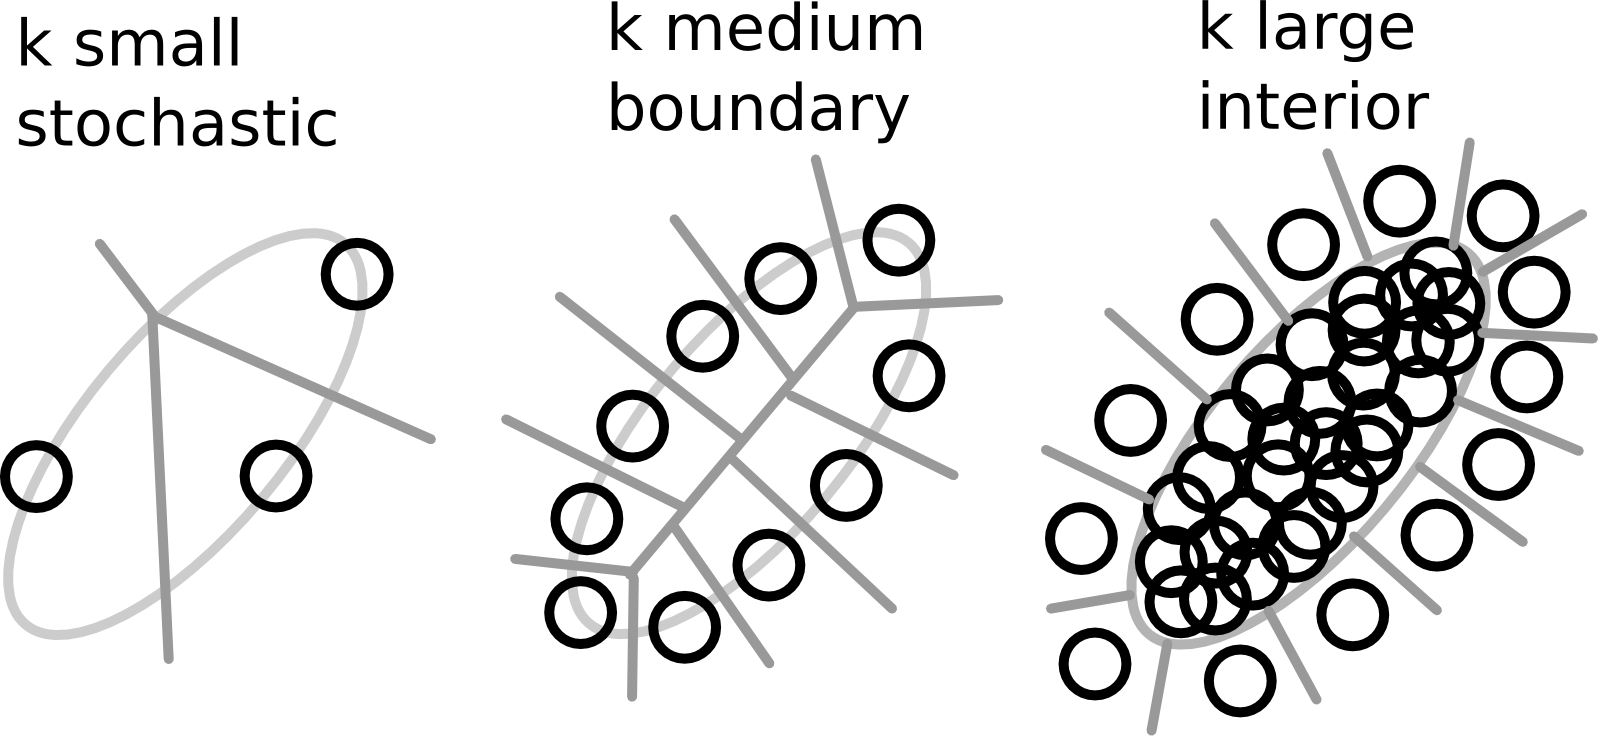
\includegraphics[scale = 0.5]{kgauss1.png}
\end{center}


\comm{
Consider independent $\vec{r}^{(1)}$ and $\vec{r}^{(2)}$ with
corresponding signal covariances $\Sigma_H^{(1)}$ and
$\Sigma_H^{(2)}$, and error covariances $\Sigma_\epsilon^{(1)}$ and
$\Sigma_\epsilon^{(2)}$.  By transforming both $\vec{r}^{(i)}$ it is
clear that we can take $\Sigma_\epsilon = I$.

TODO: See how the summary $\mathcal{I}$  behaves when combining independent vectors.

The average correct classification rate is
\begin{align*}
\text{CC} &= \Pr[||\vec{r} - \mu_1||_{\Sigma_\epsilon}^2 < \min_{j > 1} ||\vec{r} - \mu_j||_{\Sigma_\epsilon}^2 | j^* = 1]
\\&= \Pr[\forall j  > 1: \mu_j \notin B_{||\epsilon||_{\Sigma_\epsilon}}(\vec{r})]
\\&= \Pr[\mu_2 \notin B_{||\epsilon||_{\Sigma_\epsilon}}(\vec{r})]^{K - 1}
\\&= \int_{\mathbb{R}^d \times \mathbb{R}^d} \left[1 - \int_{B_{||\epsilon||_{\Sigma_\epsilon}}(r)} p(\mu) d\mu\right]^{K-1} dP(\epsilon, \vec{r})
\end{align*}
where $B_r(x)$ is the euclidean $\Sigma_\epsilon$-normed ball of radius $r$ centered at $x$ and
\[
p(\mu) = \frac{1}{(2\pi|\Sigma_\mu|)^{d/2}} \exp(-\frac{1}{2}\mu^T \Sigma_\mu^{-1} \mu)
\]
}

\subsection{Relation to information theory}

Somehow the above can be related to mutual information 
\[I(\vec{h}, \vec{r}) \propto \ln(\Sigma_H) - \ln(\Sigma_H(\Sigma_H + \Sigma_\epsilon)^{-1} \Sigma_H)\]

\subsection{Information theory facts}

Suppose
\[
\begin{pmatrix}
X \\ Y
\end{pmatrix}
\sim \mathcal{N}\left(
0, \begin{pmatrix}
\Sigma_X & \Sigma_{XY} \\
\Sigma_{YX} & \Sigma_Y
\end{pmatrix}
\right)
\]

Then, the mutual information between $X$ and $Y$ is
\[
I(X; Y) = -\frac{1}{2}\log \det[\Sigma_X^{-1/2}(\Sigma_{XY}\Sigma_Y^{-1}\Sigma_{YX})\Sigma_X^{-1/2}]
\]
while the Fisher information, treating $X$ as the parameter and $Y$ as the data, is
\[
J = \Sigma_X^{-1}(\Sigma_{XY}\Sigma_{Y|X}^{-1}\Sigma_{YX})\Sigma_X^{-1}
\]
where
\[
\Sigma_{Y|X} = \Cov(Y|X) = \Sigma_Y - \Sigma_{YX}\Sigma_X^{-1}\Sigma_{XY}
\]

Notice the similarity between $J$ and the argument of $\det$ in the mutual information.

\subsection{Robustness}

We wish to apply the methods derived using the preceding Guassian
theory to non-Gaussian case: how well does it generalize?

\subsection{Instability}

Due to natural selection, the brain is optimized to selectively
process the information from the outside world.  Compared to the
totality of information captured by the senses, only a small fraction
may be relevant to survival.  In more quantitative terms, sensory
information may be extremely high-dimensional, but the useful portion
of that information takes the form of a lower-dimensional summary.

Hence, if $S$ is high-dimensional, but the relevant information takes
the form of a low-dimensional summary $L = h(S)$, then we have $I(S;
X) = I(L; X)$.  Such a dimension-reduction assumption may be crucial
to obtaining tractable estimates of $I(S; X)$.

We argue, however, that instability issues limit the possibility of
using MI or FI in this fashion.  For the sake of illustration, suppose
we consider linear summaries $L = SA$, where $A$ is a coefficient
matrix.  For instance, $L$ may be the first $k$ principal components
of $S$.  However, now note that estimation of the principal components
(or even the number of components) is highly noisy.  Hence... [argue
that if $L$ is estimated as first principal components, $I(L; X)$ will
be highly variable for MI or FI.]


\section{Estimating Encoding Parameters}

\subsection{Previous Work}

Consider a parametric model
\[
Y \sim F_\theta(X)
\]
Such a \emph{forward model} gives the distribution of the
response conditional on the stimuli features.

The \emph{maximum likelihood} (ML) principle can be invoked to
identify the stimuli $i \in S$ ``most likely'' to have produced $y^*$.
Let $x_i : i \in S$ denote features of the test stimuli, and
identify $y^*$
\[
i^* = \text{argmax}_i \ell_\theta(y^*| x_i)
\]

\emph{Example.} We take the following as a representative approach, combining features of [1] and [2]:
\begin{itemize}
\item Assume the normal mutivariate linear model
\[Y \sim N( XB , \Sigma_E), \text{ where }B \in \mathbb{R}^{q \times p}\]
\item Estimate $B$ using elastic net [4]
\item Estimate $\Sigma_E$ using off-diagonal shrinkage of sample covariance matrix of residuals
\item The ML rule takes the form
\begin{equation}\label{mlrule}
i^* = \text{argmin}_{i} (x_i^T \hat{B} - y^*)^T \hat{\Sigma}_E^{-1} (x_i^T \hat{B} - y^*)
\end{equation}
\end{itemize}

\subsection{Emprirical Bayes Approach}

\begin{itemize}
\item \emph{Idea}: Unlike ML, the Bayes rule surely optimizes the ``correct'' objective function.  Can we approximate the Bayes rule?
\item \emph{Empirical Bayes}: use the data to estimate the covariances
$\Sigma_B$ and $\Sigma_E$, then compute posterior distribution of $B$
\item Assume coefficients of $B$ independent; diagonals of $\Sigma_B$ can be estimated using any estimate of signal strength, e.g. \emph{Eigenprism} [3].
\item Decision rule similiar to \eqref{mlrule} but with ``added noise'' due to uncertainty of $B$.
\[
\text{min} (x_i^T B - y^*)^T (\text{Cov}(x_i^T B) + \hat{\Sigma}_E)^{-1} (x_i^T B - y^*)
\]
\item Analogous to LDA vs QDA
\end{itemize}

\subsection{Covariance Estimation}

Both ML approach and EB approach depend on estimates of the covariance of $Y$.
We might assume a ``Kronecker'' model where $\Cov(Y) = \Sigma_v \times \Sigma_t$
where $\Sigma_v$ is the covariance of voxels (for a fixed time point)
and $\Sigma_t$ is the autocovariance of a given voxel.

New approaches to estimating covariance $\Sigma_v$ might incorporate
spatial information about voxel location, or functional information.

\subsection{Computation}

Suppose we have a $n \times p_Y$ response matrix $Y$ and a $n \times p_X$ covariate matrix $X$.
We have the model
$$
Y = XB + E
$$
where $B$ is a $p_X \times p_Y$ coefficient matrix and $E$ is a matrix of noise.
Write $$
E = \begin{pmatrix} e_1^T\\e_2^T\\ ... \\ e_n^T \end{pmatrix}
$$
Assume the rows of $E$ are independent, and each row is distributed
$$
e_i \sim N(0, \Sigma_e)
$$

Let us assume a prior distribution on the coefficients,
$$
B_{ij} \sim N(0, \sigma^2_{B, j})
$$
and where $B_{ij}$ are independent.
Note that each column $j = 1,...,p_Y$ has a different prior coviarance $\sigma^2_{B, j}$.
This reflects our prior knowledge that some column of $Y$ may have more signal than other columns.

Bayes' rule gives us the posterior mean and covariance of the coefficients $B_{ij}$.
First, we introduce the vectorized notation $\vec{B}$ to denote the $p_X p_Y \times 1$ vector obtained by 
stacking the columns of $B$, and similarly $\vec{Y}$ to denote the $p_Y n \times 1$ vector obtained by stacking the columns of $Y$.  Also recall the definition of Kronecker product,

$$
A \otimes B = \begin{pmatrix}a_{11} B & a_{12} B & ...\\
a_{21} B & a_{22} B & ...\\
... & ... & ...\end{pmatrix}
$$

Also define
$$
\Omega_e = \Sigma_e^{-1}
$$
$$
\Omega_b = \text{diag}\left(\frac{1}{\sigma^2_{b, 1}},..., \frac{1}{\sigma^2_{b, p_Y}}\right)
$$

The posterior mean and covariance are given as follows.

$$
\text{E}[\vec{B}|Y] = (\Omega_e \otimes X^T X + \Omega_b \otimes I_{p_X})^{-1} ((I\otimes X)^T (\Omega_e \otimes I) \vec{y})
$$
$$
\text{Cov}(\vec{B}|Y) = = (\Omega_e \otimes X^T X + \Omega_b \otimes I_{p_X})^{-1}
$$

Given a new observation $y_* = B^T x_* + e_*$, where $y_*$ and $x_*$ are column vectors,
the posterior predictive distribution is
$$
\text{E}[y_* | Y] = (I_{p_Y} \otimes x_*^T) \text{E}[\vec{B}|Y]
$$
$$
\text{Cov}[y_* | Y] = (I_{p_Y} \otimes x_*^T) \text{Cov}(\vec{B}|Y) (I_{p_Y} \otimes x_*) + \Sigma_e
$$


In the following, we assume that $p_X > n$.

Naively, computing the posterior covariance takes $O(p_X^3 p_Y^3)$ operations
and computing the posterior mean takes $O(p_X^2 p_Y^2)$ operations.

However, by diagonalizing the covariance matrix and taking advantage of the properties of Kronecker products, we can make the computation much more efficient.

Using simultaneous diagonalization, find $V_e, D_e$ such that
$$
\Omega_e = V_e D_e V_e^T
$$
and
$$
\Omega_b = V_e V_e^T
$$
Note that $V_e$ is not orthogonal.
The procedure for finding $V_e, D_e$ is well-known and also given in the code.

Furthermore, define 
$$\tilde{X} = \begin{pmatrix} X \\ 0\end{pmatrix}$$ so that $\tilde{X}$ is an $p_X \times p_X$ matrix.
Then take the SVD
$$
\tilde{X} = U_X D_X V_X^T
$$
so that $D_X$ and $V_X$ are both  $p_X \times p_X$.
We have
$$
V_X V_X^T = V_X V_X^T = I_{p_X}
$$
and
$$
V_X D_X^2 V_X^T = X^T X.
$$

Now we can rewrite the expression
$$
\text{Cov}(\vec{B}|Y) = = (\Omega_e \otimes X^T X + \Omega_b \otimes I_{p_X})^{-1}
$$
$$
= ((V_e D_e V_e^T) \otimes (V_X D_X^2 V_X^T) + (V_e V_e^T) \otimes (V_X V_X^T))^{-1}
$$
$$
= [(V_e \otimes V_X) (D_e \otimes D_X^2+ I_{p_X p_Y})(V_e^T \otimes V_X^T)]^{-1}
$$
$$
= (V_e^{-1} \otimes V_X^{T})^T (D_e \otimes D_X^2+ I_{p_X p_Y})^{-1} (V_e^{-1} \otimes V_X^{T})
$$

In this form the expression is much each to compute since
\begin{itemize}
\item Only a diagonal matrix needs be inverted, and yields a diagonal matrix
\item Multiplying the tranpose of a Kronecker product with a diagonal with itself is easy to compute.
\end{itemize}
To see the second point, consider computing the product

$$
C = (A \otimes B)^T D (A \otimes B)
$$
where $A$ is $a_1 \times a_2$, $B$ is $b_1 \times b_2$, and $D$ is diagonal with
$$
D = \begin{pmatrix} D_1 & 0 & 0 & 0 &... \\
0 & D_2 & 0 & 0 & ...\\
0 & 0 & D_3 & 0 & ...\\
... & ...& ... & ... & ...
\end{pmatrix}
$$
such that each $D_1,..., D_{a_1}$ is $b_1 \times b_1$.

For $i, j = 1..., a_2$, let $C_{[ij]}$ denote $b_2 \times b_2$ blocks such that
$$
C = \begin{pmatrix} C_{[11]} & C_{[12]} & ...\\
C_{[21]} & C_{[22]} & ... \\
... & ... & ...\end{pmatrix}
$$

Now we can write
$$
C_{[ij]} = \sum_{k=1}^{a_1} a_{ki}a_{kj} B^T D_k B 
= \left(\sum_{k=1}^{a_1} a_{ki} a_{kj} B^T D_k B \right)
= B^T \left(\sum_{k=1}^{a_1} a_{ki} a_{kj} D_k \right) B.
$$

The second-to-last and last equality present two alternative methods to compute $C_{[ij]}$.

\begin{itemize}
\item Using the second-to-last equality, one precomputes each of the matrices $B^T D_i B$, which takes $O(b_2^2 b_1 a_1)$ operations.  To compute each block, it takes $O(b_2^2 a_1)$ operations.  Hence, to compute $C$ takes $O(a_1 a_2^2 b_2^2)$.
\item Using the last equality, for each block one takes $O(a_1 b_1)$ operations to compute the weighted sum of $D_1,..., D_{a_1}$, and then $O(b_2^1 b_1)$ to multiply on the left with $B^T$ and on the right with $B$.
\end{itemize}
Therefore, we see that it takes $O(a_2^2 b_2^2 b_1)$ operations to compute $C$.

Choosing the best of the two methods, the cost to compute $C$ is $O(a_2^2 b_2^2 \min(a_1, b_1))$.
Applying to our problem, we see that the cost to evaluate the posterior covariance using this method is $O(p_Y^2 p_X^2 \min(p_X, p_Y))$, which is a saves a factor of $\max(p_Y, p_X)$ compared to the naive approach.


\section{Inferring Information Content}

\subsection{Finite Sample Effect}

Changing slightly the notation, let $\text{MC}(\vec{r}, K, n)$ denote
the misclassification when classifying $K$ random classes, given a
training set of size $n$.  Our definition of information is computed
from $\text{MC}(\vec{r}, K, \infty)$: the misclassification curves
assuming a \emph{known} encoding rule.  However, in practice, we only
know $\text{MC}(\vec{r}, K, n)$ for finite $n$.

\subsection{Learning Curves}

The question is whether one can estimate $\text{MC}(\vec{r},
K, \infty)$ based on knowing $\text{MC}(\vec{r}, K, n)$ for various
$n \leq N$, where $N$ is the total number of observations available.

Cortes et al propose the following method to model the training and
test error as a function of $n$, the training set size:

\[
\text{Err}_{\text{train}} = a - \frac{b}{n^\beta}
\]
\[
\text{Err}_{\text{test}} = a + \frac{c}{n^\alpha}
\]
where $a$, $b$, $c$, $\alpha$ and $\beta$ are to be determined
empirically.

GOAL: Extend this type of empirical model to also incoporate $K$, the
number of test classes, and justify somehow.

\subsection{Two-class problem}

Suppose $\mu_1, \mu_2 \sim N(0, \Sigma)$, and $Y_i \sim N(\mu_i, I)$.
What is the misclassification rate, i.e.
\[
MC(\Sigma, 2) = \Pr[||Y_1 - \mu_1||^2 > ||Y_1 - \mu_2||^2]
\]
Without loss of generality, assume $\Sigma = \diag(\lambda_1,\hdots, \lambda_d)$.
Let $X = Y_1 - \mu_1$ and $D = \mu_1 - \mu_2$.
Then $X \sim N(0, I)$ and $D \sim N(0, 2\Sigma)$, where $X$ and $D$ are independent, and we have
\begin{align*}
MC(\Sigma, 2) &= \Pr[||X||^2 > ||X + D||^2]
\\&= \Pr\left[\sum_{i=1}^d X_i^2 > \sum_{i=1} (X_i + D_i)^2]\right]
\\&= \Pr\left[-2 \sum_{i=1}^d D_i X_i > \sum_{i=1} D_i^2]\right]
\\&= \E\left[\Pr\left[-2 \sum_{i=1}^d D_i X_i > \sum_{i=1} D_i^2]\right]|D\right]
\end{align*}
where we have conditioned on $D$.  Let $S = \sum_{i=1} D_i^2$.
Then conditional on $D$, we have $\sum_{i=1}^d D_i X_i \sim N(0, S)$, meaning that
\[
\Pr\left[-2 \sum_{i=1}^d D_i X_i > \sum_{i=1} D_i^2]|D\right] = \Pr[N(0, 4S) > S|D] = 1-\Phi(\sqrt{S/4})
\]
hence
\[
MC(\Sigma, 2) = 1 - \E \Phi(\sqrt{S}/2)
\]

\subsection{High-dimensional asymptotics}

Here we consider the limit $MC(\Sigma_d, k)$, for a sequence $\Sigma_d$ with
the appropriate limit properties.

\textbf{Theorem.}
There exists a function $m(c, k)$ for $c > 0$, and $k \in \{1, 2, \hdots\}$, such that
\[
m(c, k) = \lim_{d \to \infty} MC(\Sigma_d, k)
\]
for all sequences of covariance matrices such that 
$$\lim_{d \to \infty} \tr \Sigma_d = c$$
and also 
$$\lim_{d \to \infty} \tr \Sigma_d^2 = 0$$

\emph{Proof.}
Note that for $\mu \sim N(0, \Sigma)$, we have
\[
\E ||\mu||^2 = \tr \Sigma
\]
and
\[
\Var ||\mu||^2 = 2 \tr\Sigma^2
\]
Hence, the fact that $\tr \Sigma_d \to c$ and $\tr \Sigma_d^2 \to 0$ imply that
for arbitrary $\epsilon > 0$, we can find $d$ sufficiently large such that with probability greater than $1-\epsilon$,
\[
\max_{1 \leq i \leq j \leq k} \langle \mu_i, \mu_j \rangle < \epsilon
\]
and
\[
\max_{1 \leq i \leq k} |||\mu_i||^2 - c| < \epsilon
\]
for $\mu_1,\hdots, \mu_k \sim N(0, \Sigma_d)$.
Let $A$ denote the event in which both inequalities hold.

In the event $A$, 
\[
\mu_i = \sqrt{c} e_i + O(\epsilon)
\]
given an appropriate orthonormal basis $e_1,\hdots, e_k$.

Similar to before, we have
\[
MC(\Sigma_d, k) = \Pr[||\mu_1 - Y_1||^2 > \min_i ||\mu_i - Y_1||^2]
\]
where $Y_1 \sim N(\mu_1, I)$.

Let us write
\[
Y_1 - \mu_1 = \sum_i Z_i e_i,
\]
and in the event $A$, we have
\[
Y_1 - \mu_i = \sum_i Z_i e_i + \sqrt{c}e_1 - \sqrt{c}e_i + O(\epsilon)
\]

It follows that
\begin{align*}
MC(\Sigma_d, k) =& \Pr[||\mu_1 - Y_1||^2 > \min_i ||\mu_i - Y_1||^2]
\\=& \Pr[A]\Pr[||\mu_1 - Y_1||^2 > \min_i ||\mu_i - Y_1||^2|A] \\&+ \Pr[A^c]\Pr[||\mu_1 - Y_1||^2 > \min_i ||\mu_i - Y_1||^2|A^c]
\\=& \Pr[||\mu_1 - Y_1||^2 > \min_i ||\mu_i - Y_1||^2|A] + O(\epsilon)
\\=& \Pr[2\sqrt{c}Z_1 > \min_i 2\sqrt{c}Z_i + 2c + O(\epsilon)] + O(\epsilon)
\\=& \Pr[\min_i (Z_i + O(\epsilon)) < Z_1 - \sqrt{c}] + O(\epsilon)
\intertext{noting that the function $\Pr[\min_i (Z_i + \xi_i) < Z_1 - \sqrt{c}]$ is continuous and jointly differentiable with respect to $\xi_i$
 at $\xi = 0$,}
=& \Pr[\min_i Z_i < Z_1 - \sqrt{c}] + O(\epsilon)
\\=&  1 - \int_{\mathbb{R}} \Phi(\sqrt{c} - z)^{k-1} d\Phi(z) + O(\epsilon)
\end{align*}


Hence in the limit,
\[
\lim_{d \to \infty} MC(\Sigma_d, k) = 1 - \int_{\mathbb{R}} \Phi(\sqrt{c} - z)^{k-1} d\Phi(z)
\]

\subsection{High-SNR limit}

Rather than fixing the number of classes $K$ and increasing the
dimension, we could also derive a limit by fixing the dimensionality
and increasing both the signal covariance $\Sigma$ and the number of
classes $K$.  The difference between the high-SNR limit and the
high-dimensional limit is that the dimensionality of the space will
influence the asymptotics.

Recall that we define $MC(\Sigma, k)$ by the misclassification given
that that joint distribution of a class center $\mu$ and a member of the class $Y$ is
\[
\begin{pmatrix}
\mu \\
Y
\end{pmatrix}\sim N\left(0, \begin{pmatrix}
\Sigma & \Sigma\\
\Sigma & \Sigma + I
\end{pmatrix}\right)
\]

In the high-SNR limit, it is notationally more convenient to consider an different parameterization.
Defining $\Omega=\Sigma^{-1}$, one can compute $MC(\Sigma, K)$ as the misclassification rate
of the model where
\[
\begin{pmatrix}
\mu \\
Y
\end{pmatrix}\sim N\left(0, \begin{pmatrix}
I & I\\
I & I + \Omega
\end{pmatrix}\right)
\]

Let $k = K-1$.  To compute the misclassification rate, we draw from
the joint distribution of $(\mu^*, Y, \mu_1,\hdots, \mu_k)$ where
$\mu^*,\mu_1,\hdots, \mu_k \sim N(0, I)$ and $Y \sim N(\mu^*, \Omega)$,
and then compute
\[
MC(\Sigma, K) = \Pr[\min_{i=1}^k ||Y - \mu_i||^2_\Sigma < ||Y - \mu^*||^2_\Sigma]
\]
under the specified joint distribution, where
\[
||x||_\Sigma^2 = x^T \Sigma x = x^T\Omega^{-1}x.
\]
We sample in the following way.  First, draw $Y \sim N(0, I
+ \Omega)$.  Then draw $\mu^* \sim N((I+\Omega)^{-1}Y,
I-(I+\Omega)^{-1})$ and $\mu_1,\hdots, \mu_k \sim N(0, I)$.
Conditioning on $Y = y$, $Y - \mu^*$ is independent of $Y - \mu_1,\hdots, Y - \mu_n$:
defining $A = I-(I + \Omega)^{-1}$, we have
\[
\begin{pmatrix}
y - \mu^*\\
y - \mu_1\\
\vdots\\
y - \mu_k
\end{pmatrix} \sim N\left(
\begin{pmatrix}
Ay\\
y\\
\hdots\\
y
\end{pmatrix},
\begin{pmatrix}
A & 0 & \cdots &0\\
0 & I & \cdots &0\\
0 & \vdots & \cdots & 0\\
0 & 0 & \cdots &I
\end{pmatrix}
\right)
\]

Thus, we are computing
\[
MC(\Sigma, K) = \E_Y[\Pr[\min_{i=1}^k ||y + Z_i||^2_\Sigma < ||Ay + A^{1/2} Z^*||^2_\Sigma]|Y=y]
\]
where $Z^*,Z_1,\hdots, Z_k$ are iid $N(0, I)$.

%Eventually, we will look for limiting sequences of $(y, \Sigma, K, a,
%b)$, where $a$ and $b$ are scaling constants, defining $M
%= \min_{i=1}^k ||y + Z_i||^2_\Sigma$ and $V = ||Ay + A^{1/2}
%Z^*||^2_\Sigma$, we have that $aM + b$ converges in probability to a
%constant while $aV + b$ converges to a Gaussian distribution.
%Hence under such a limit, $MC(\Sigma, K)$ converges to a constant.

To prepare for such a result, we approximate the distribution of $M$ when $\Sigma$ and $y$ are large.
The $p$th quantile of $M$ is the $1-(1-p)^{1/k}$th quantile of $||y + Z_i||^2$.
For large $\Sigma$, we can approximate
\[
\Pr[||y+ Z_i||^2_\Sigma < x] \approx \phi_d(y) \det(\Sigma)^{-1/2}\Vol(B_d(\sqrt{x})) = 
\phi_d(y) \sqrt{\det(\Omega)} \frac{2(\pi x)^{d/2}}{d\Gamma(d/2)}
\]
where $B_d(r)$ is the euclidean ball with radius $r$ and $\phi_d(y) = (2\pi)^{-d/2} e^{-||y||^2/2}$.
Hence, the $p$th quantile of $M$ is $x_p$ where
\[
x_p \approx \frac{1}{\pi}\left(
\frac{d\Gamma(d/2)}{2} \frac{(-\log(1-p)/L)\sqrt{\det(\Sigma)}}{\phi_d(y)}
\right)^{2/d}
\]
Upper and lower bounds for the approximation are given in the appendix.
%In order for the variance of $M$ to vanish it must be the case that
%$x_\epsilon$ and $x_{1-\epsilon}$ are close for some small $\epsilon$.
%In order for this to be the case, we must have $L$ sufficiently large so that
%\[
%\left(\frac{-\log(\epsilon)}{L} \sqrt{\det{\Sigma}}\right)^{2/d} 
%\]
%is small.


Let us now turn to the distribution of $V$.
We have $A \to \Omega$ in the limit of large $\Sigma$.
Then,
\[
||Ay + A^{1/2}Z||^2_\Sigma \approx ||\Omega y + \Omega^{1/2}Z||^2_\Sigma = ||\Omega^{1/2} y + Z||^2
\]

\section{Appendix}

\subsection{Approximation bounds for high-SNR limit}

For $x > 0$ we have
\[
K(\Sigma)x^{d/2}\phi_d(\underline{y})< \Pr[||y+Z_i||^2_\Sigma < x] < K(\Sigma)x^{d/2}\phi_d(\overline{y})
\]
and
\[
\left(\frac{1-\sqrt[L]{1-p}}{K(\Sigma)\phi_d(\overline{y})}\right)^{2/d}
< x_p < 
\left(\frac{1-\sqrt[L]{1-p}}{K(\Sigma)\phi_d(\underline{y})}\right)^{2/d}
\]
where
\[
K(\Sigma) = \sqrt{\det(\Omega)} \frac{2\pi^{d/2}}{d\Gamma(d/2)}
\]
and $\overline{y}, \underline{y}$ are to be derived as follows.

Consider the optimization problems
\[
\text{minimize or maximize} ||z-y||^2 \text{subject to}||z||_\Sigma^2 \leq \epsilon
\]
We assume $\epsilon$ sufficiently small such that the the solutions
satisfy the hard constraint $||z||_\Sigma^2 = \epsilon$.  Both the
minimization and maximization problems are solved by taking the
Lagrangian
\[
||z-y||^2 + \lambda z^T \Sigma z
\]
and setting the derivative equal to zero:
\[
0 = 2z - 2y + 2\lambda\Sigma z
\]
yielding
\[
z = (I- \lambda \Sigma)^{-1}y.
\]
The constrained extrema are obtained by solving for $\lambda$ in the constraint:
\[
\epsilon = y^T(I-\lambda\Sigma)^{-1}\Sigma(I-\lambda\Sigma)^{-1}y
\]
Letting $\lambda_1,\lambda_2$ be the two roots, we have 
\[\{\overline{y}, \underline{y}\} = \{y - (I- \lambda_1 \Sigma)^{-1}y, y - (I- \lambda_1 \Sigma)^{-1}y\}\]
which can be disambiguated by the fact that $||\overline{y}|| < ||\underline{y}||$.


\end{document}



